\documentclass[10pt]{article}

\usepackage[margin=1in]{geometry}
\usepackage{graphicx}
\usepackage{amsmath}
%\usepackage[colorlinks,bookmarks,bookmarksnumbered,allcolors=blue]{hyperref}
\usepackage{booktabs}   % For better tables
\usepackage{caption}
\usepackage{cleveref}
\usepackage{enumitem}   % For shorteneted itemize list
\usepackage{titling}    % To adjust title placement

\begin{document}

\title{Wind Farm Layout Optimization Case Study 3
\\
\small{IEA Task 37 on System Engineering in Wind Energy}
}
\author{\large Nicholas F. Baker,\  Andrew P. J. Stanley, \ and Andrew Ning \\
    {\small Brigham Young University, Provo, Utah, USA}\\
\vspace{-1em}\\
\large Katherine Dykes\\
    \small National Renewable Energy Laboratory, Golden, Colorado, USA}
\setlength{\droptitle}{-5em}
\maketitle

\section{Introduction}

    Two major factors that affect wind farm layout optimization are 1) the optimization approach and 2) the wake model.
    We have thus far conducted two case studies to analyze differences in these variables, this document defines a third and fourth case study to further study these factors when given more realistic wind farm boundaries.
    Case study 3 presents a scenario with a concave boundary.
    Case study 4 presents a scenario with both concave boundaries and discontinuous boundary regions.
    For case studies 3 and 4, the user is free to choose both optimization approach and wake model.

    Participants will (1) optimize turbine locations to maximize annual energy production, (2) submit solutions with details regarding their optimization convergence and methodology.
    After all submissions are received, participants will be expected to perform a cross comparison of other participant solutions.
    Data will be consolidated, processed, and made available to all participants.

\section{Problem Definition}

    \subsubsection*{Objective}

        The objective of each scenario is to maximize annual energy production, which we define simply as the expected value of aerodynamic power.
        For case studies 3 and 4, the wind resource is given as a continuous Weibell distribution, and participants are free to use as many $n$ directional bins as they wish.
        In other words:
        \begin{equation*}
            AEP = \left(\sum_{i=1}^{n} f_i P_i\right) 8760 \frac{\textrm{hrs}}{\textrm{yr}}
        \end{equation*}
        where $P_i$ is the power produced for wind direction $i$, and $f_i$ is the corresponding wind direction probability.

    \subsubsection*{Design Variables}

        The design variables are the $(x, y)$ locations of each turbine, all $z$ values will be the same in these case studies.
        All locations in this document refer to the hub location.
        Every turbine in the farm is identical, and explicitly defined below in \textbf{Parameters}.

    \subsubsection*{Constraints}

        In case studies 1 and 2, all farm boundaries were uniformly circular and centered on the origin.
        To make these studies more realistic, the boundaries are non-uniform, and case study 4 is made up of discontinous regions.
        It is based on the Borselle III and IV wind farms, depicted graphically in \Cref{fig:cs3-boundary,fig:cs4-boundary} and with coordinates in \texttt{iea37-cs3-boundary.yaml} and \texttt{iea37-cs4-boundary.yaml}.
        All turbine rotors ($(x, y)$ locations + rotor radius) must remain completely on or within this boundary.
        No turbine hub can be less than two rotor diameters from any other hub.

        %begin{figure}[]
        %    \begin{center}
        %    \includegraphics[width=2.6in]{iea37-cs3-boundary.png}
        %    \caption{Graphic depicton of wind farm boundary}
        %    \label{fig:boundary}
        %    \end{center}
        %\end{figure}

        \begin{minipage}[c]{0.49\textwidth}
            \centering
            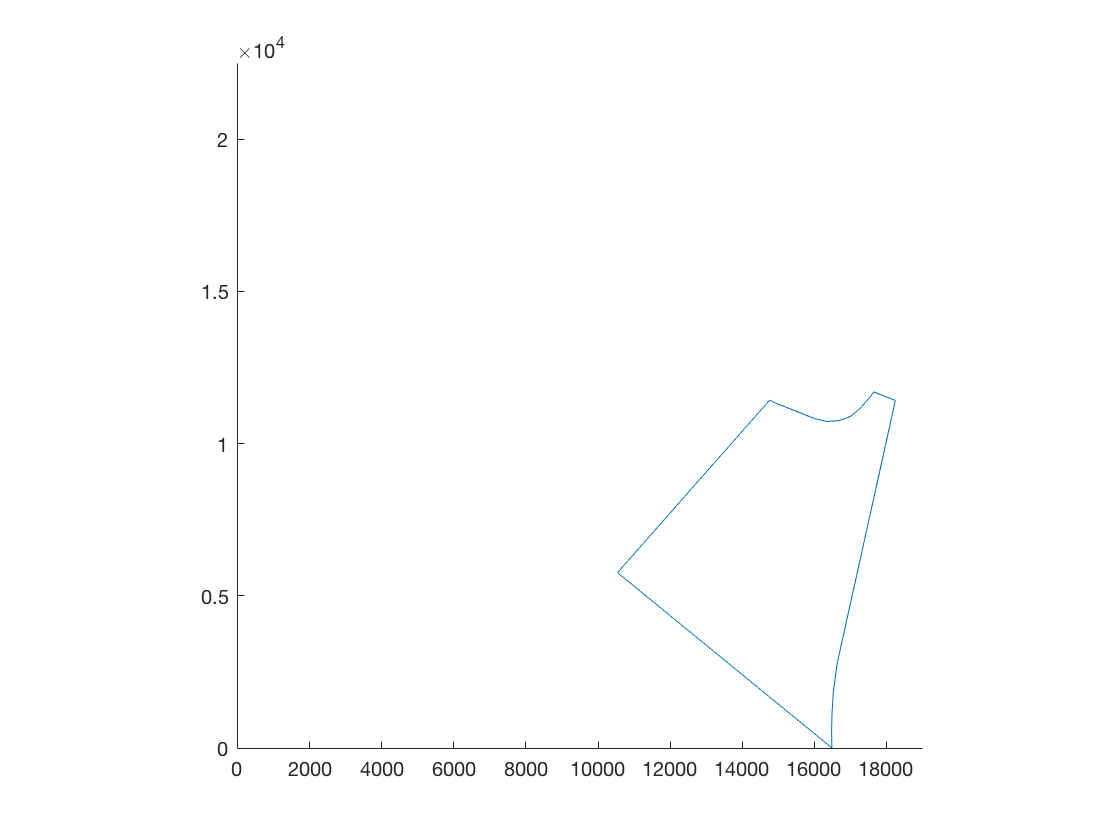
\includegraphics[width=3.25in]{cs3-boundary.png}
            \captionof{figure}{Graphic depicton of wind farm boundary for case study 3}
            \label{fig:cs3-boundary}
        \end{minipage}\quad
        \begin{minipage}[c]{0.49\textwidth}
            \centering
            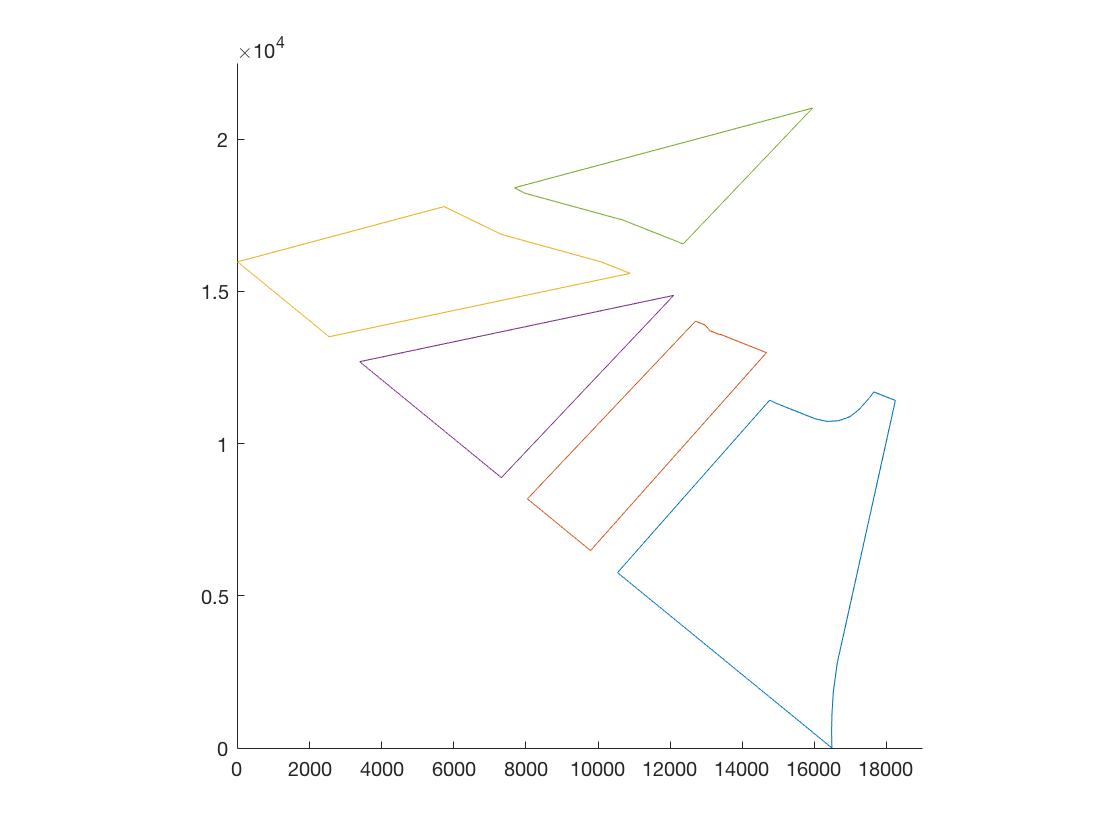
\includegraphics[width=3.25in]{cs4-boundary.png}
            \captionof{figure}{Graphic depicton of wind farm boundary for case study 4}
            \label{fig:cs4-boundary}
        \end{minipage}

    \subsubsection*{Parameters}

        The wind turbine is the IEA37 10 MW offshore reference turbine \cite{NREL10MW} with the following characteristics:
        \begin{center}
            \begin{tabular}{@{}lrl@{}}
            \toprule
                Rotor Diameter & 198.0 & m \\ 
                Turbine Rating & 10 & MW \\ 
                Cut-In Wind Speed & 4 & m/s \\ 
                Rated Wind Speed & 11 & m/s \\ 
                Cut-Out Wind Speed & 25 & m/s \\
            \bottomrule
            \end{tabular}
        \end{center}

        \noindent All turbine data is also contained in the enclosed \texttt{iea37-10mw.yaml}. The power curve is defined as:   

        \begin{minipage}{0.53\textwidth}
            \begin{equation*}
                P(V) = 
                \begin{cases} 
                    0 & V < V_{\textit{cut-in}} \\
                    P_{\textit{rated}}\cdot\bigg(\frac{V-V_{\textit{cut-in}}}{V_{\textit{rated}}-V_{\textit{cut-in}}}\bigg)^3 & V_{\textit{cut-in}}\leq V < V_{\textit{rated}} \\
                    P_{\textit{rated}} & V_{\textit{rated}} \leq V < V_{\textit{cut-out}} \\
                    0 & V \geq V_{\textit{cut-out}}
                \end{cases}
            \label{eq:power}
            \end{equation*}
        \end{minipage}\quad
        \begin{minipage}{0.53\textwidth}
            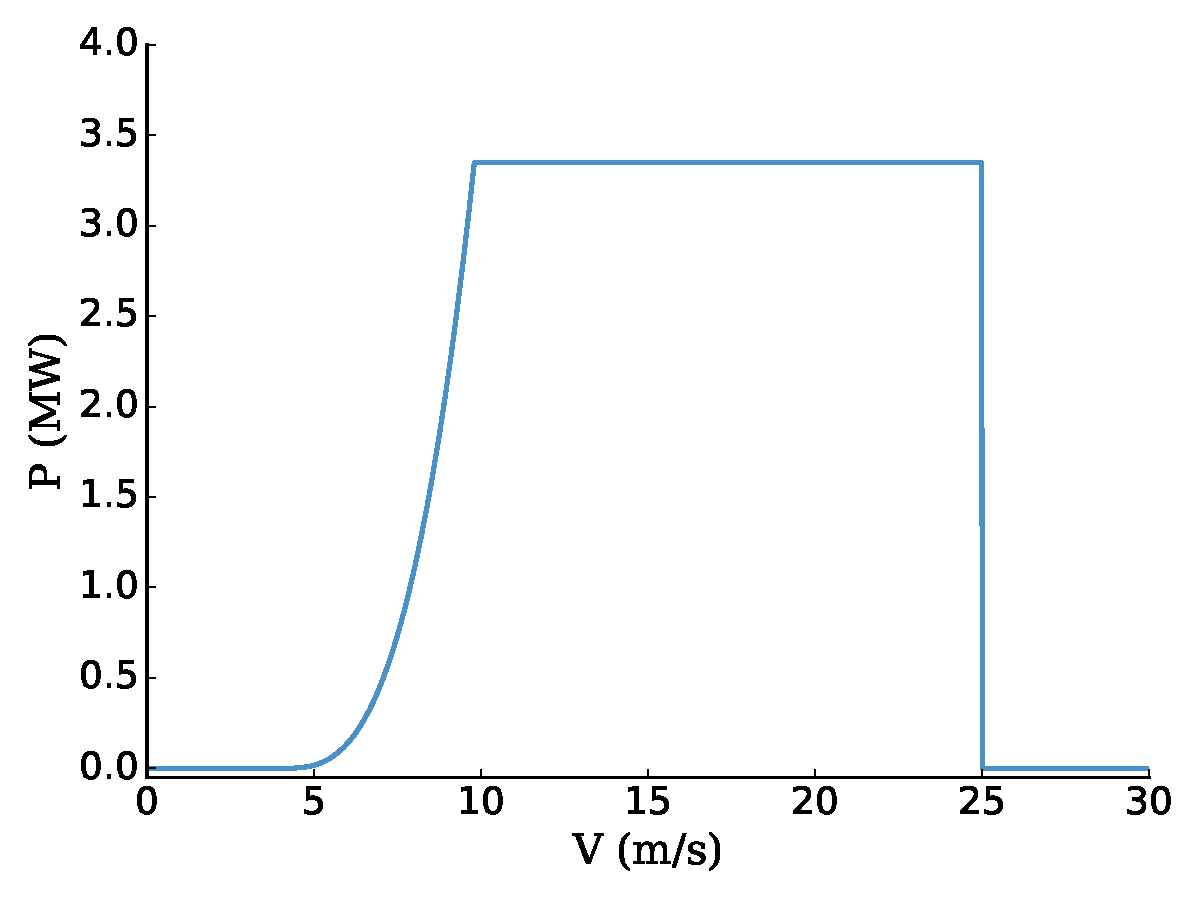
\includegraphics[width=2.6in]{iea37-335mw-pcurve}
        \end{minipage}

        The farm wind speed for all scenarios is constant at 9.8 m/s. The \texttt{+}y axis is coincident with $0^{\circ}$, and the CW wind rose is defined by 16 discrete bins tabulated in \texttt{iea37-windrose.yaml}, depicted pictorially below:
       %\vspace{-4.5em}
        \begin{center}
            %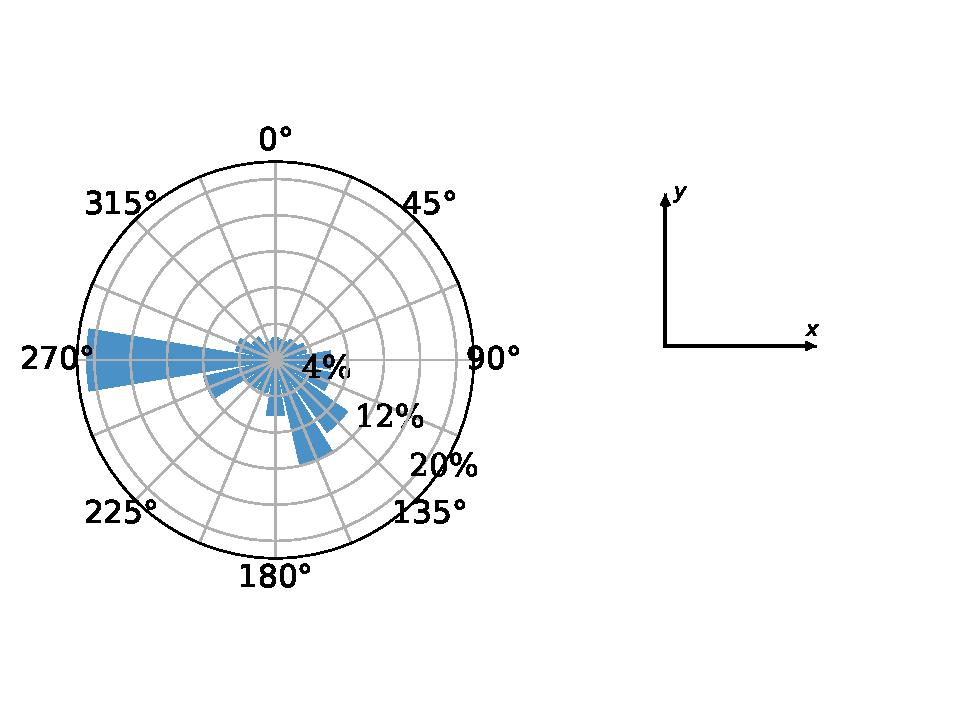
\includegraphics[width=5in]{iea37-windrose-axis}
        \end{center}
        %\vspace{-5em}
    \subsection{Baseline Layouts}

        Since both the files supplied to users necessary for participation, as well as the resulting output provided by each participant are in very precise formats, baseline layouts for both case studies are supplied.
        These files are called \texttt{iea37-cs3-baseline.yaml} and \texttt{iea37-cs4-baseline.yaml}.
        Like the example layouts provided for case studies 1 and 2, this baseline layouts are meant to provide a reasonable minimum output against which results can be measured.
        Participants are not required to use the baseline layouts as starting points for their optimizations, though they are permitted to do so.
        
        Users participating in case studies 3 and 4 will use their own wake model (thus the specific model-computed AEP values in the \texttt{.yaml} files will vary), but the baseline layouts are supplied as example submissions, to understand the specific \texttt{.yaml} reporting format we require.

    \subsection{Case Study 3}

        This problem defines a scenario where the user is free to choose both the optimization algorithm and the wake model.
        This single wind farm scenario is twenty-five (25) turbines with a boundary containing concavities.
        It is graphically depicted in \cref{fig:cs3-boundary} and defined in \texttt{iea37-cs3-boundary.yaml}.
    
    \subsection{Case Study 4}

        This problem adds discontinuous boundary regions to the problem presented in case study 3.
        The user is free to choose both the optimization algorithm and wake model.
        It is requested that participants use the same algorithm and model that they used in case study 3 in order for us to observe scalability differences, but users are not required to do so.
        This single wind farm scenario is eighty-one (81) turbines with a boundary containing concavities and discontinuities.
        The boundaries for case study 4 are graphically depicted in \cref{fig:cs4-boundary} and defined in \texttt{iea37-cs4-boundary.yaml}.

\section{Reporting and Evaluation}

    Participants will submit:
    \begin{enumerate}
        \item Optimal turbine placement solution using the \texttt{.yaml} format from the enclosed baseline layout. 
        \item Optimization performance and timing metrics using the \texttt{.yaml} format from the enclosed baseline layouts.
    \end{enumerate}

    Note that your \texttt{.yaml} submissions must report both total farm AEP, and farm AEP for each of you chosen binned wind directions, as in the enclosed \texttt{iea37-cs\#-baseline.yaml} examples.

    \subsection{Reporting}

        Since results will be analyzed mainly through cross-comparison, submissions must adhere to the \texttt{.yaml} format in order to receive a ranking.
        Submitted files should be named:
        
        \vspace{0.5em}
        \texttt{\$iea37-cs\#-yourname.yaml}
        \vspace{0.5em}
        
        \noindent Where: 
        \begin{itemize}
            \item ``\texttt{cs\#}'' is the case study number of the submission (``cs3'' or ``cs4'').
            \item ``\texttt{yourname}'' is your personal or organizational name, all lowercase with no spaces or punctuation.
        \end{itemize}

        \noindent The following two files must be referenced internally by your submission, as is done by the baseline layout:
        \begin{itemize}
            \item \texttt{iea37-cs3-windrose.yaml} describes the Weibel distribution wind rose used in both case studies.
            \item \texttt{iea37-10mw.yaml} lists the turbine data for the used IEA37 10 MW offshore reference turbine.
            \item \texttt{iea37-cs\#-boundary.yaml} which gives the point outline of the wind farm boundaries.
        \end{itemize}

        As shown in the example results given in \texttt{iea37-cs\#-baseline.yaml} files, timing and intermittent AEP calculations will be required.
        This means each participant must log the intermittent AEP calculations through the optimization process, to track convergence data.
        Plots will be made to observe how quickly each algorithm and model pairing converges to a solution.
    
    \subsection{Evaluation}
        Because the participant wake models are intended to differ, determining a ``best'' solution is generally not possible.
        Comparisons will be made using two approaches:
        \begin{enumerate}
            \item Every participant will evaluate every other participant's solutions using their own wake model(s).  It is essential that the \texttt{.yaml} format is adhered to so that cross-comparisons are painless. % If the optimizations behave as expected, each participant's wake model will judge their own solution as best, but it is possible a solution is found that other wake models agree is better.
            \item Each solution will be compared using a higher-fidelity simulation, in this case large-eddy simulations (LES) using SOWFA.  This simulation introduces its own modeling assumptions and is an imperfect way to compare, but does provide another piece of information on relative performance between approaches. % It is expected that solutions with minor LES performance differences would lie within the error of the methodology, and thus only major differences will be used in drawing conclusions on relative performance.
        \end{enumerate}

\section{Enclosures}
    Files included with this document, needed for full participation in the case studies are:

    \begin{itemize}[noitemsep,topsep=0pt,parsep=0pt,partopsep=0pt]
        \item \texttt{iea37-cs3-windrose.yaml} - the same for both \texttt{cs3} and \texttt{cs4}, a continuous Weibull distribution in \texttt{.yaml} format
        \item \texttt{iea37-cs3-10mw.yaml} - data for reference turbine used in both case studies, in \texttt{.yaml} format
        \item \texttt{iea37-cs3-boundary.yaml} - the coordinates of the wind farm's boundary for case study 3
        \item \texttt{iea37-cs4-boundary.yaml} - the coordinates of the wind farm's boundary for case study 4
        \item \texttt{iea37-cs3-baseline.yaml} - example optimization results, denoting timing and iteration analysis
    \end{itemize}

\bibliographystyle{aiaa}
\bibliography{iea37-wflocs-announcement}

\end{document}